\documentclass[12pt]{report}

% Language setting
% Replace `english' with e.g. `spanish' to change the document language
\usepackage[english,russian]{babel}	

% Set page size and margins
% Replace `letterpaper' with `a4paper' for UK/EU standard size
\usepackage[letterpaper,top=2cm,bottom=2cm,left=3cm,right=3cm,marginparwidth=1.75cm]{geometry}

% Useful packages
\usepackage{amsmath}
\usepackage{amssymb}
\usepackage{graphicx}
\usepackage[colorlinks=true, allcolors=blue]{hyperref}
\usepackage{fancyhdr}

\title{\huge МКЭ}
\author{\huge Подлесов Егор}

\date{}

\begin{document}
\fancyhead{}
\fancyhead[C]{\huge СВТ: МКЭ}
\maketitle
\thispagestyle{fancy}


\section{Постановка задачи}
В области $\Omega = [0, 1]^2$ решается двумерная задача Дирихле для двумерного стационарного оператора диффузии: 
\begin{center}
    \begin{cases}
    (-\mathbb{D} u) = f, x \in \Omega,\\
    u|_{\delta \Omega} = g, 
    \end{cases}
\end{center}
где $\mathbb{D} = diag(d_x, d_y)$. Для решения используется Метод конечных элементов на треугольной сетке $w_h = ih, jh$, где $h = \frac{1}{N}.$


\section{Результаты экспериментов}
Рассмотрим задачи с известным аналитическим решением и построим для них графики $C$-нормы и $L_2$-нормы при измельчении сетки:
\begin{enumerate}
    \item $f = sin(\pi x)sin(\pi y)$\\
    $d_x = 1, d_y = 1$ \\
    $u = \frac{sin(\pi x)sin(\pi y)}{2\pi^2}$
    \begin{figure}[h]
        \begin{center}
        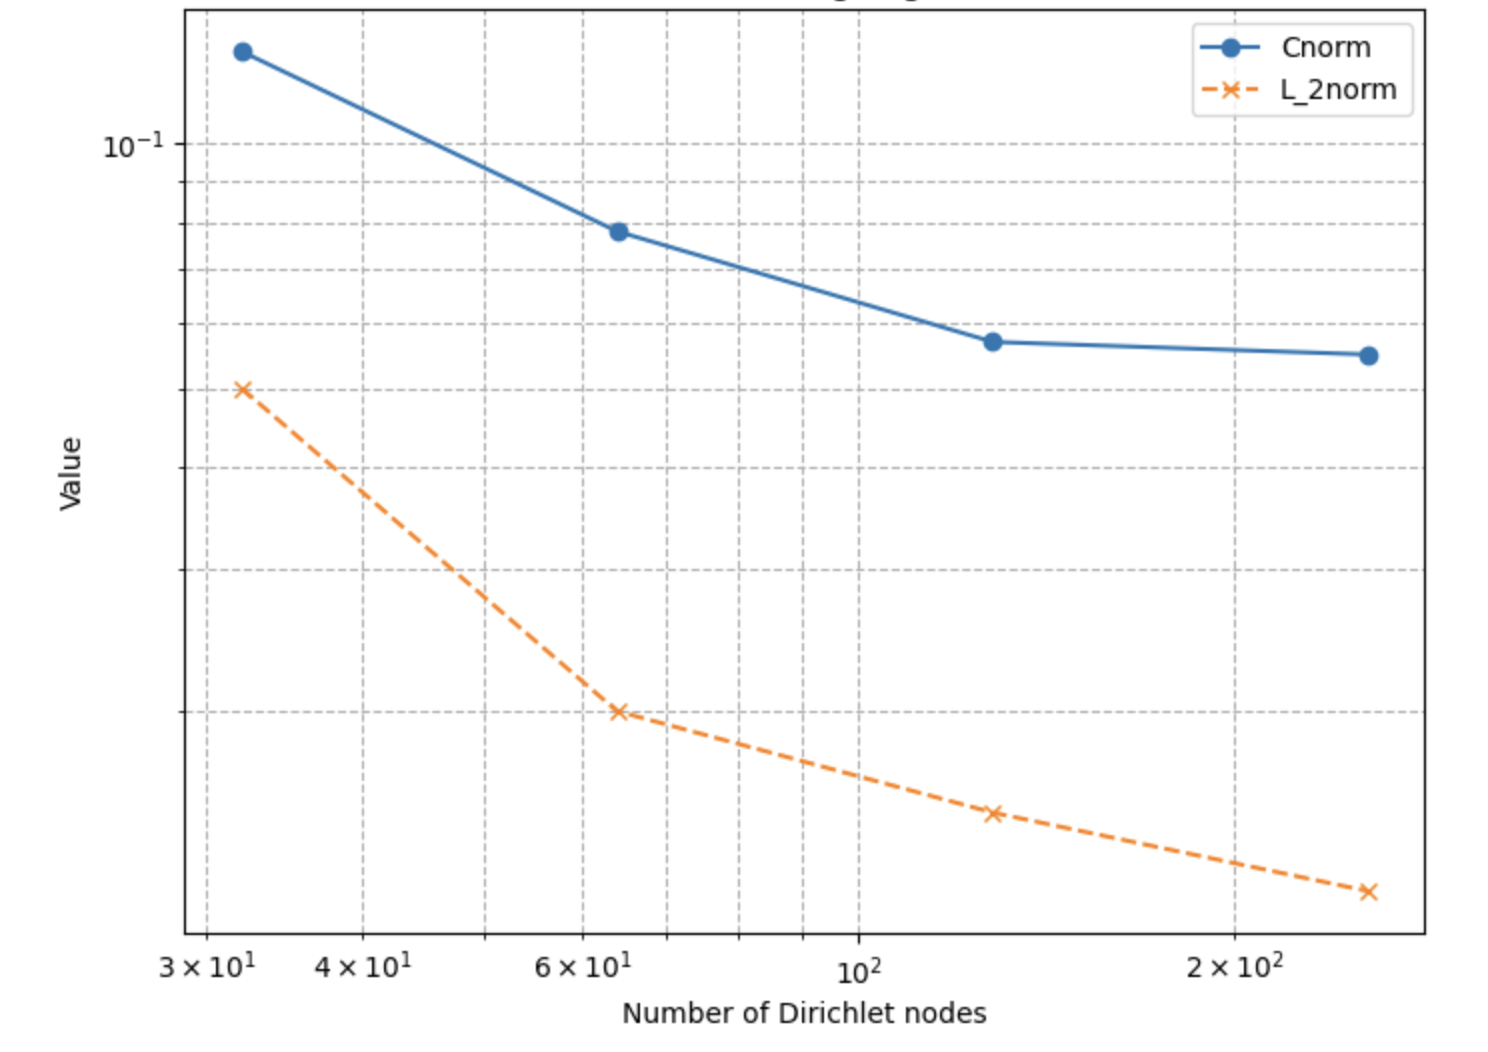
\includegraphics[scale=0.4]{gr_2.1.png}
        \caption{$f = sin(\pi x)sin(\pi y)$}
        \end{center}
    \end{figure}
    \newpage
    \item $f = sin(4 x)sin(4 y)$\\
    $d_x = 5, d_y = 1$ \\
    $u = \frac{sin(4x)sin(4y)}{16(d_x+d_y)}$
    \begin{figure}[h]
        \begin{center}
        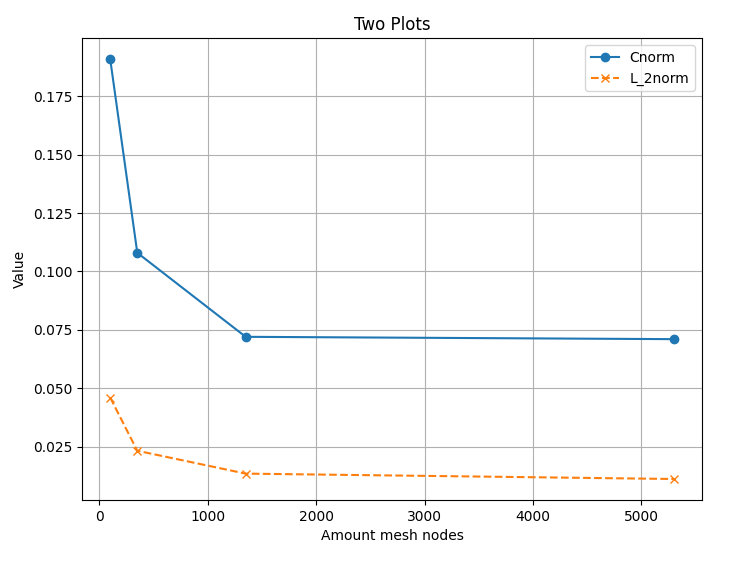
\includegraphics[scale=0.4]{gr_2.2.png}
        \caption{$f = sin(4x)sin(4y)$}
        \end{center}
    \end{figure}
\end{enumerate}

\end{document}